\documentclass[11pt]{article}
\usepackage[top=1in, bottom=1in, left=1in, right=1in]{geometry}

\usepackage{amsmath}
\usepackage{amssymb}
\usepackage{graphicx}

\title{Quiz \#7, 10/15 \\ Math 156 (Calculus I), Fall 2024}
\date{}

\begin{document}

\maketitle

\thispagestyle{empty}

\vspace{-1.75cm}

Problem 1 is worth 5 points and Problem 2 is worth 5 points, for a total of 10 points. Remember to \emph{show your work} on all problems!

\begin{enumerate}
\item Consider the curve in the plane defined by $x^3 + y^3 = x - y$. The curve is graphed below:
\vspace{-0.45cm}
\begin{center}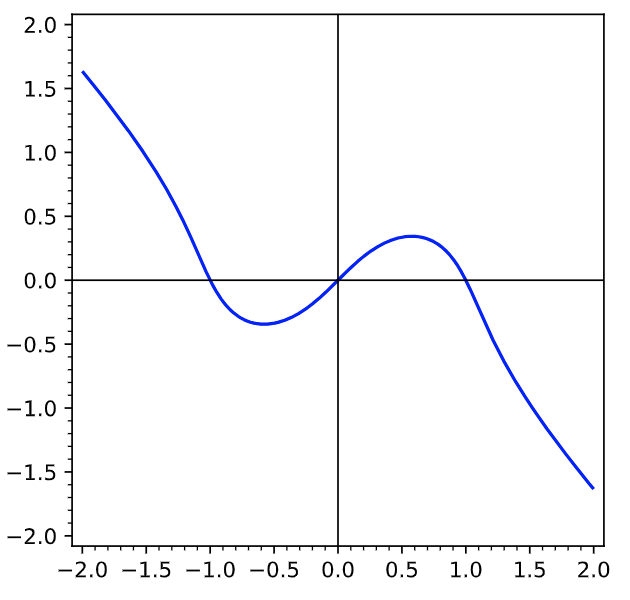
\includegraphics[width=1.75in]{quiz7.png}\end{center}
\vspace{-0.7cm}
Find the slope of the tangent line to this curve at the point $(x,y)=(-1,0)$.

\vspace{6.75cm}

\item The area of a circular bacterial colony is growing at a rate of $5$ square centimeters per day. At what rate is the radius growing when the radius is $10$ centimeters? \\{\bf Hint}: Recall that the area $A$ and radius $r$ of a circle are related by the formula $A=\pi r^2$.
\end{enumerate}

\end{document}